\documentclass{beamer}
\usepackage{tcolorbox}
\usepackage{hyperref}
\usepackage{../notation} % Custom package

%\beamerdefaultoverlayspecification{<+->}
% \newcommand{\data}{\mathcal{D}}
% \newcommand\Item[1][]{%
% 	\ifx\relax#1\relax  \item \else \item[#1] \fi
% 	\abovedisplayskip=0pt\abovedisplayshortskip=0pt~\vspace*{-\baselineskip}}

\graphicspath{ {imgs/} }

\usetheme{metropolis}           % Use metropolis theme


\title{Decision Trees : Regression}
\date{\today}
\author{Nipun Batra and teaching staff}
\institute{IIT Gandhinagar}

\begin{document}
	\maketitle
	
	\begin{frame}{Example 1}
	Let us consider the dataset given below
	\begin{center}
	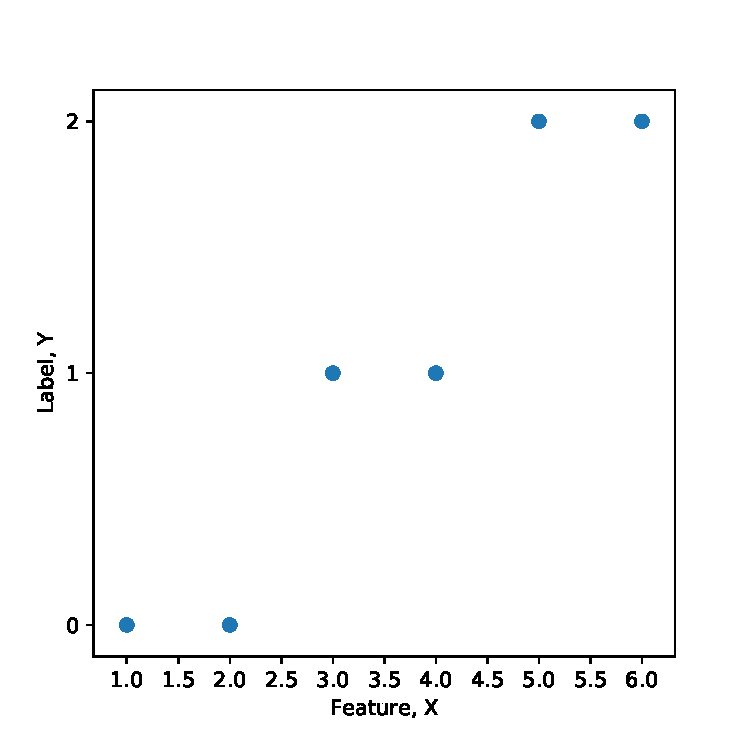
\includegraphics[scale=0.5]{dataset}
	\end{center}
	\end{frame}

	\begin{frame}{Example 1}
	What would be the prediction for decision tree with depth 0?
	\begin{center}
	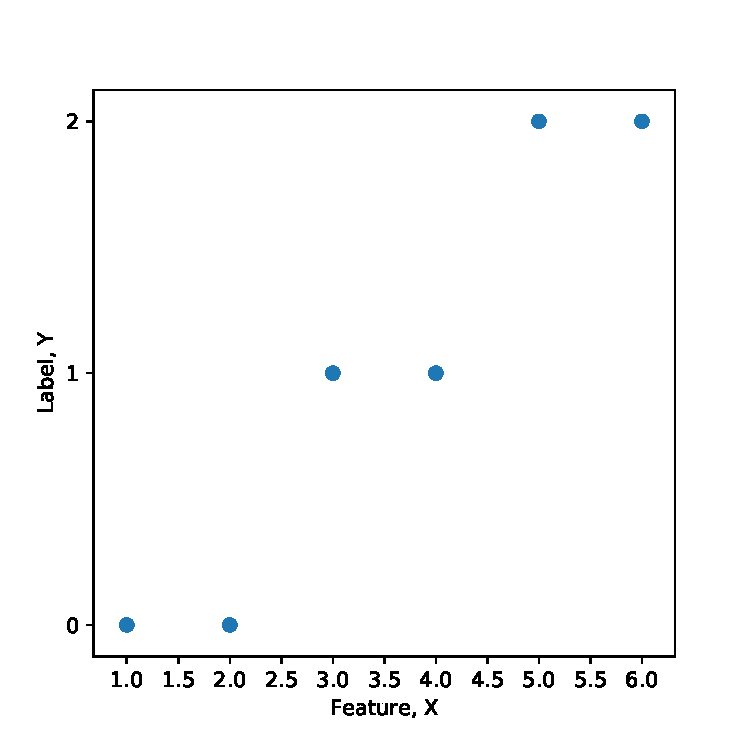
\includegraphics[scale=0.5]{dataset}
	\end{center}
	\end{frame}

	\begin{frame}{Example 1}
	Prediction for decision tree with depth 0.\\
	Horizontal dashed line shows the predicted $Y$ value. It is the average of $Y$ values of all datapoints.\\
	\begin{center}
	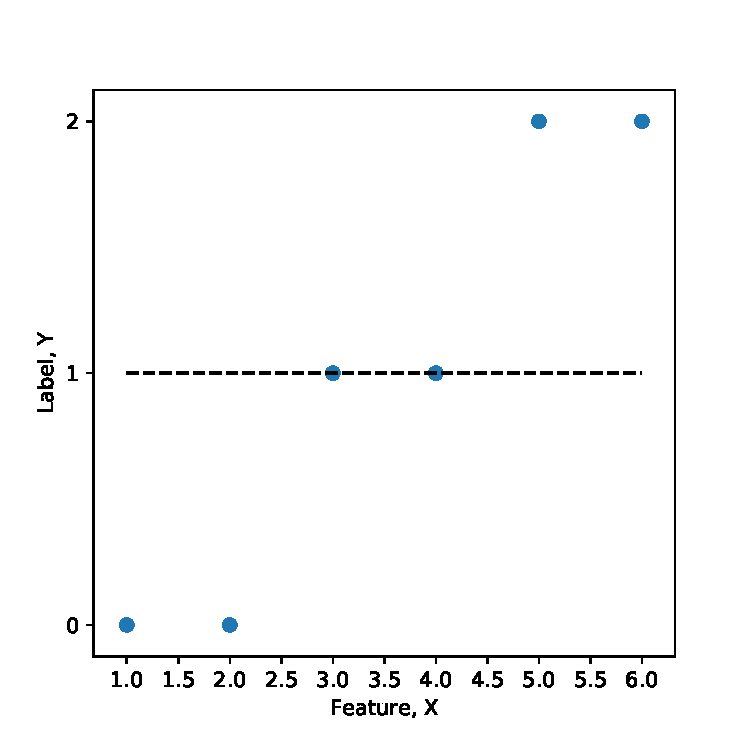
\includegraphics[scale=0.5]{depth-0-boundary}	
	\end{center}
	\end{frame}


	\begin{frame}{Example 1}
	What would be the decision tree with depth 1?
	\begin{center}
	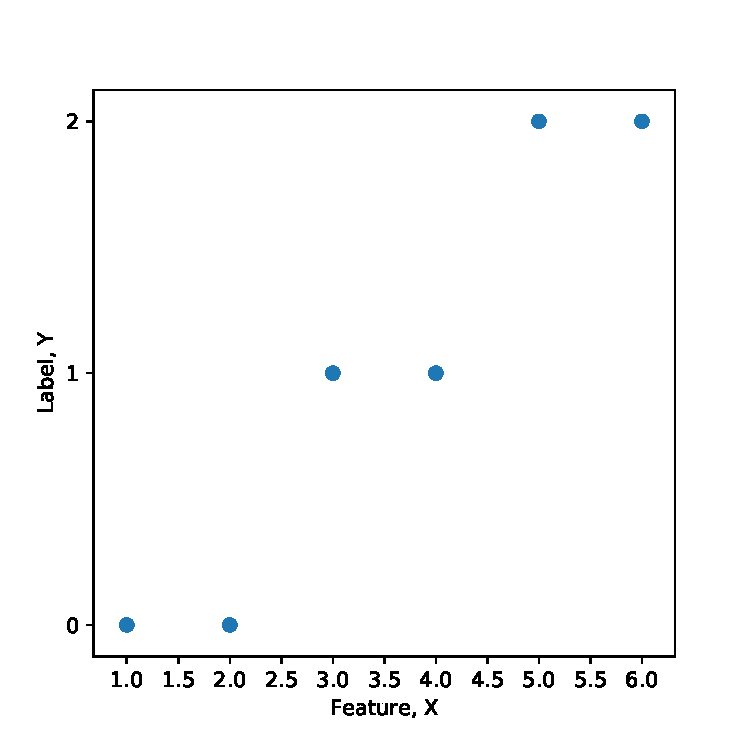
\includegraphics[scale=0.5]{dataset}
	\end{center}
	\end{frame}

	\begin{frame}{Example 1}
	Decision tree with depth 1
	\begin{center}
	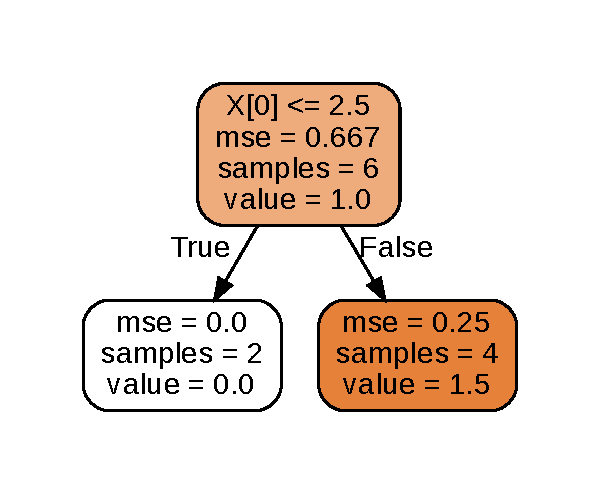
\includegraphics[scale=1]{depth-1-decision-tree}	
	\end{center}
	\end{frame}

	\begin{frame}{Example 1}
	The Decision Boundary
	\begin{center}
	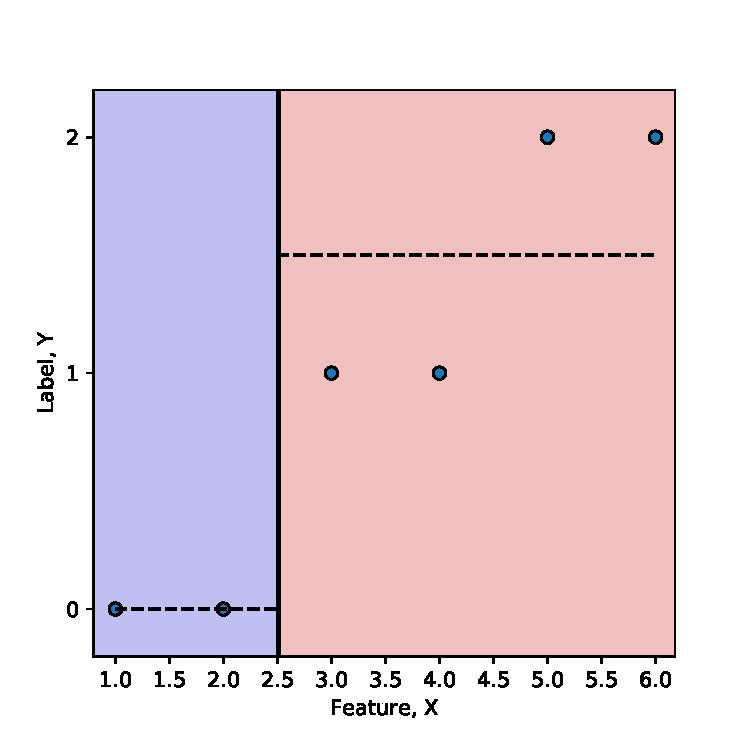
\includegraphics[scale=0.5]{depth-1-tree}
	\end{center}
	\end{frame}


	\begin{frame}{Example 1}
	What would be the decision tree with depth 2	?
	\begin{center}
	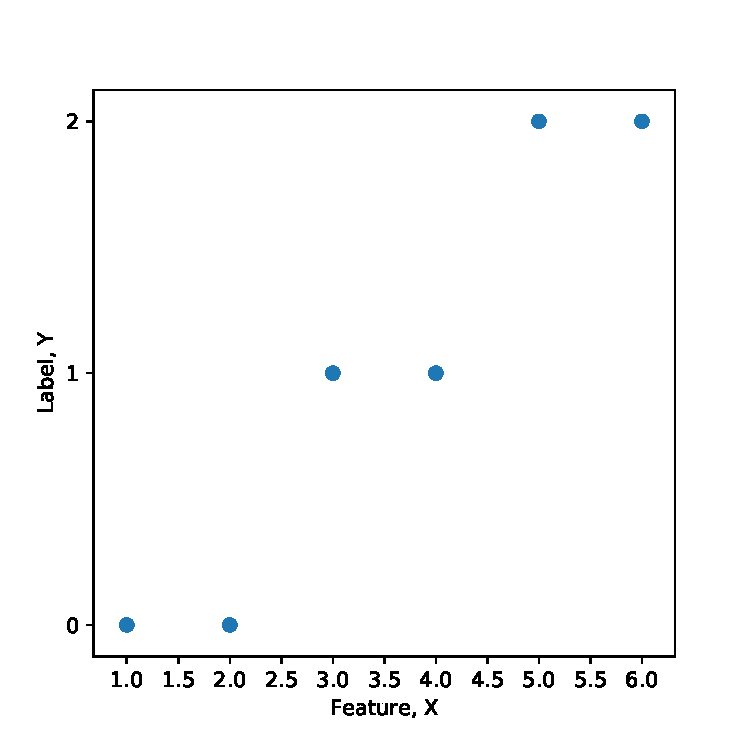
\includegraphics[scale=0.5]{dataset}
	\end{center}
	\end{frame}

	\begin{frame}{Example 1}
	Decision tree with depth 2
	\begin{center}
	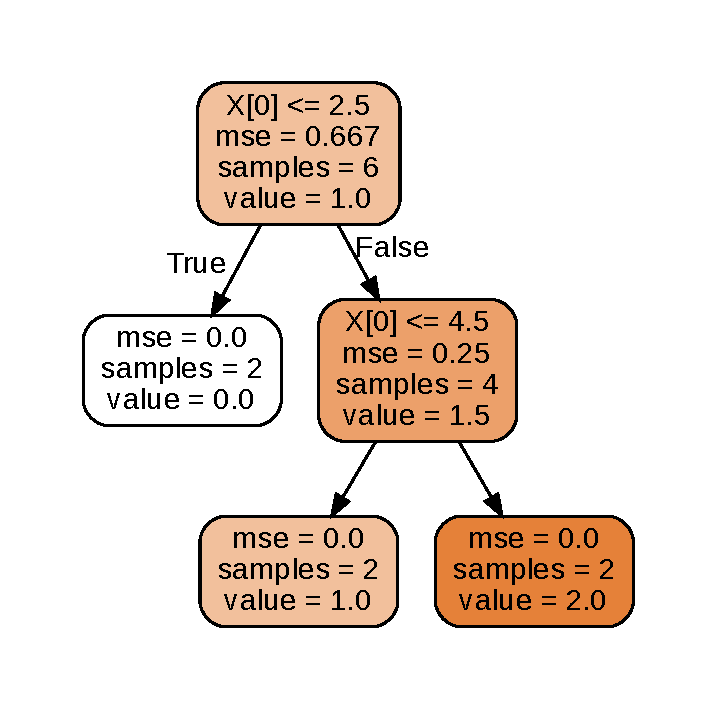
\includegraphics[scale=0.65]{depth-2-decision-tree}	
	\end{center}
	\end{frame}

	\begin{frame}{Example 1}
	The Decision Boundary
	\begin{center}
	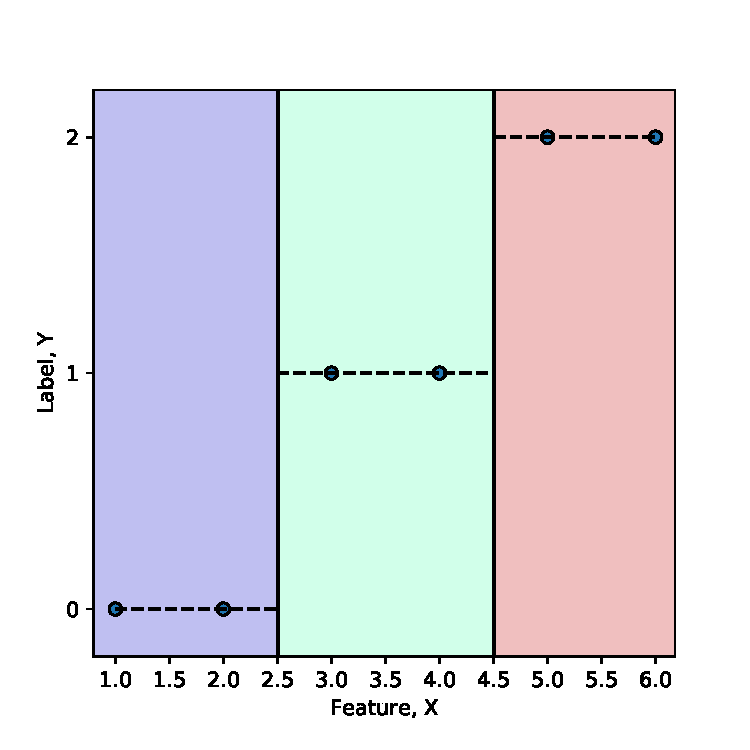
\includegraphics[scale=0.5]{depth-2-tree}
	\end{center}
	\end{frame}

	\begin{frame}{Loss function}
	\only<1-4>{
	Here,  Feature is denoted by X and Label by Y.\\
	Let the ``decision boundary'' or ``split" be at X = S.\\
	Let the region X $<$ S, be region R$_1$.\\
	Let the region X $>$ S, be region R$_2$.\\
	\vspace{1cm}
	}
	\only<2-4>{
	Then, let \\
	$C_1$ = Mean ($Y_i | X_i \in R_1$) \\
	$C_2$ = Mean ($Y_i | X_i \in R_2$) \\
	}
	\only<3-4>{
	Loss = $\sum\limits_i$(($Y_i - C_1 | X_i \in R_1$)$^2 $ +  ($Y_i - C_2 | X_i \in R_2$)$^2 $)\\
	\vspace{1cm}
	}
	\only<4>{
	Our objective is to minimize the loss and find\\
	$min_S $ $\sum\limits_i\left((Y_i - C_1 | X_i \in R_1)^2  +  (Y_i - C_2 | X_i \in R_2)^2 \right)$
	}
	\end{frame}

	\begin{frame}{How to find optimal split ``S"?}
	\end{frame}


	\begin{frame}{How to find optimal split ``S"?}
	\begin{enumerate}
	\only<1-2>{
	\item Sort all datapoints (X,Y) in increasing order of X.
	\vspace{0.5cm}
	}
	\only<2>{
	\item Evaluate the loss function for all\\
	\vspace{0.25cm}
	\begin{center}
	$S = \frac{X_i + X_{i+1}}{2}$\\
	\end{center}
	\vspace{0.25cm}
	and the select the S with minimum loss.
	}
	\end{enumerate} 
	\end{frame}

	\begin{frame}{A Question!}
	Draw a regression tree for Y = sin(X), $0 \leq X \leq 2\pi$ 
	\end{frame}

	\begin{frame}{A Question!}
	Dataset of Y = sin(X), $0 \leq X \leq 7$ with 10,000 points 
	\begin{center}
	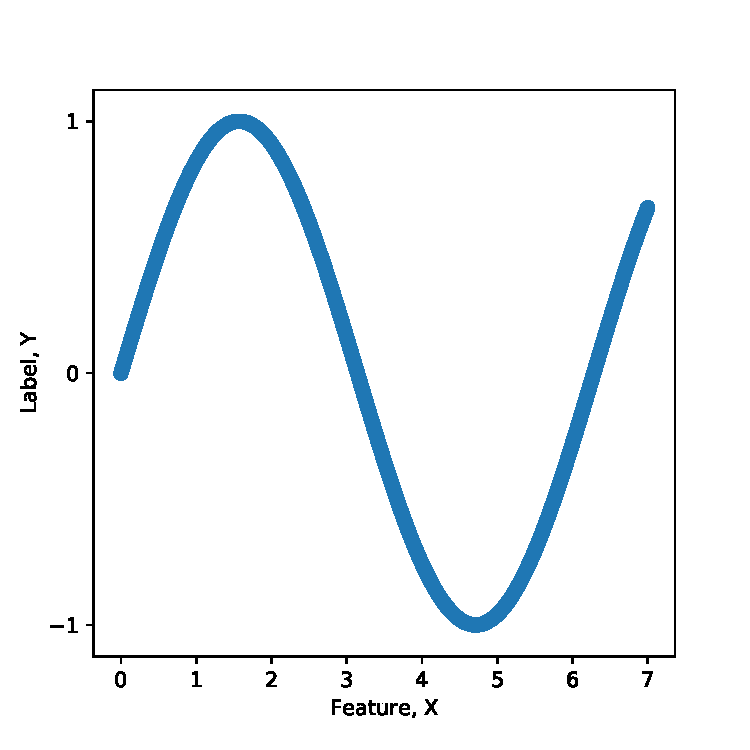
\includegraphics[scale=0.5]{sine-dataset}
	\end{center}
	\end{frame}

	\begin{frame}{A Question!}
	Regression tree of depth 1
	\begin{center}
	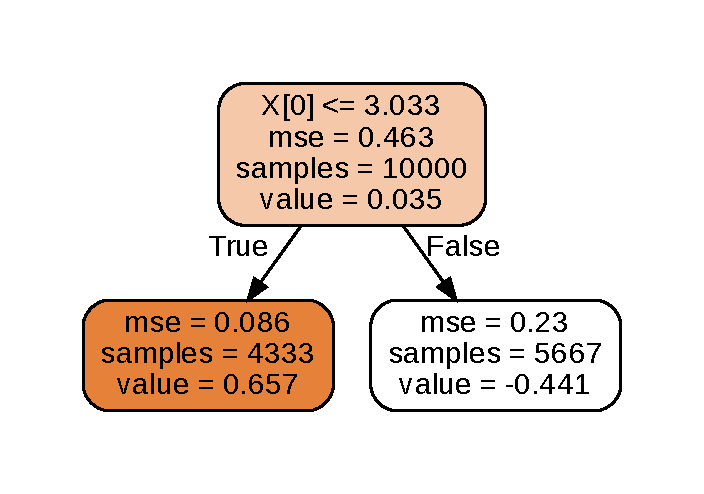
\includegraphics[scale=0.5]{sine-depth-1-decision-tree}
	\end{center}
	\end{frame}

	\begin{frame}{A Question!}
	Decision Boundary
	\begin{center}
	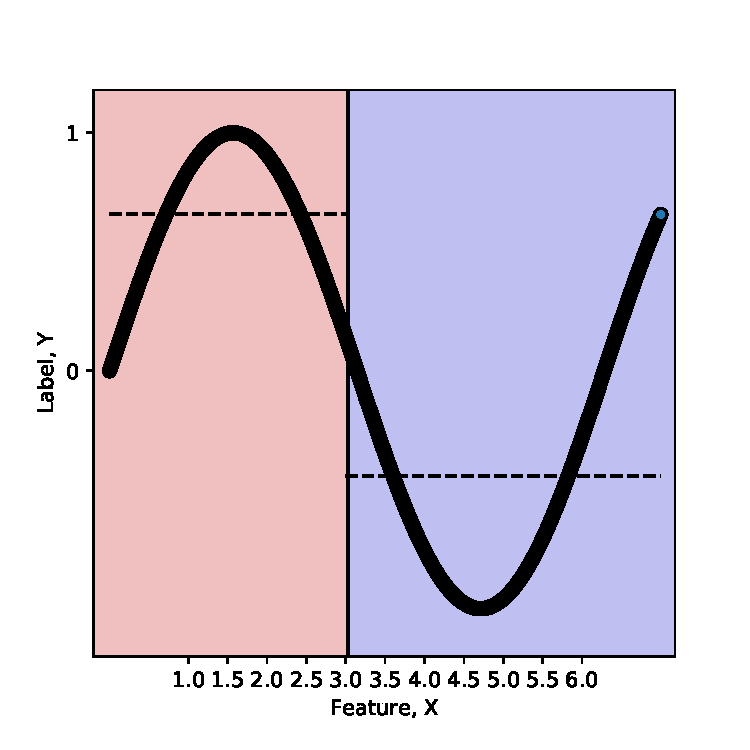
\includegraphics[scale=0.5]{sine-depth-1-tree}
	\end{center}
	\end{frame}

	\begin{frame}{A Question!}
	Regression tree with no depth limit is too big to fit in a slide. \\
	It has of depth 20. The decision boundaries are in figure below.\\
	\begin{center}
	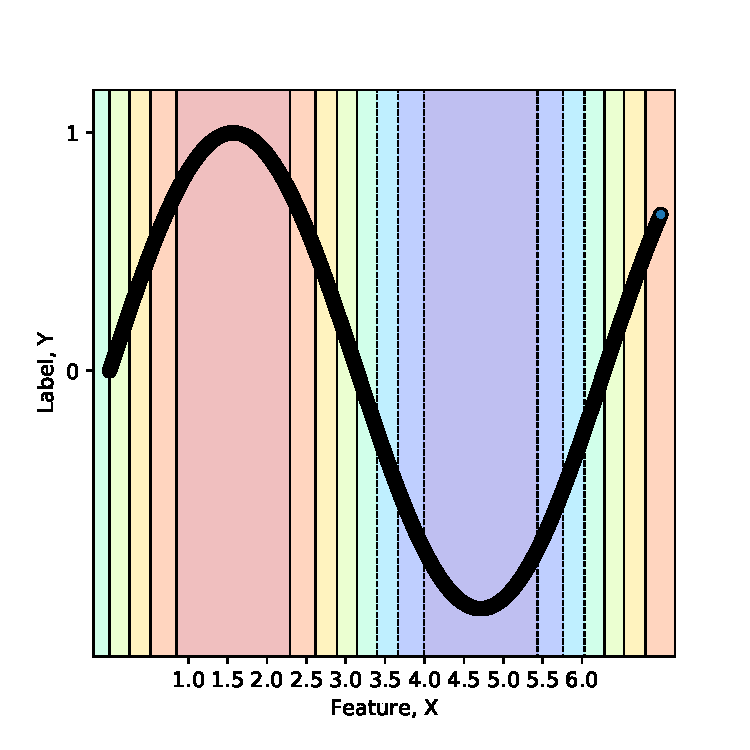
\includegraphics[scale=0.5]{sine-no-depth-tree}
	\end{center}
	\end{frame}

	\begin{frame}{Code for examples}
	\begin{center}
	\href{https://colab.research.google.com/drive/1NnuVxypYfEOvpMbFHE4075CI-EkT8S7B}{Google Colab}
	\end{center}
	\end{frame}

\end{document}